\textbf{Ejemplo 8}\\
Hallar el valor presente de 15 egresos que crecen en un 25\%pav, si el primer egreso es de  800.000 COP y suponiendo una tasa del 20\% periódica anual vencida.\\

	%%%%%%%%%%%%%%%%%%% EJERCICIO 8 %%%%%%

%\newpage %USAR SOLO SI EL SOLUCIÓN QUEDA SOLO Y ES NECESARIO BAJARLO A LA SIGUIENTE PAGINA
\textbf{Solución.}\\
%La tabla ira centrada
\begin{center}
	\renewcommand{\arraystretch}{1.6}% Margenes de las celdas
	%Creación de la cuadricula de 3 columnas
	\begin{longtable}[H]{|c|c|c|}
		%Creamos una linea horizontal
		\hline
		%Definimos el color de la primera fila
		\rowcolor[HTML]{FFB183}
		%%%%% INICIO ASIGNACIÓN FECHA FOCAL %%%%%%%
		%%%%%%%%%% INICIO TITULO
		%Lo que se hace aquí es mezclar las 3 columnas en una sola
		\multicolumn{3}{|c|}{\cellcolor[HTML]{FFB183}\textbf{1. Asignación período focal}}  \\ \hline
		\multicolumn{3}{|c|}{$pf = \textit{0 pav}$}   \\\hline
		%%%%%%%%%% FIN TITULO
		%%%%% INICIO DECLARACIÓN DE VARIABLES %%%%%%%
		%%%%%%%%%% INICIO TITULO
		%Lo que se hace aquí es mezclar las 3 columnas en una sola
		\multicolumn{3}{|c|}{\cellcolor[HTML]{FFB183}\textbf{2. Declaración de variables}}   \\ \hline
		%%%%%%%%%% FIN TITULO
		%%%%%%%%%% INICIO DE MATEMÁTICAS
		%Cada & hace referencia al paso de la siguiente columna
		
		\multicolumn{2}{|c|}{$\hspace{2 cm}R=   800{.}000COP \hspace{2 cm}$} & $g=25\% \textit{de incremento entre serie geometrica con } g \neq i$ \\
		\multicolumn{2}{|c|}{$\hspace{2 cm}n=15 \textit{ pav} \hspace{2 cm}$} & $i=20\% \textit{ pav}$ \\
		\multicolumn{2}{|c|}{$\hspace{2 cm}VP= ? COP   \hspace{2 cm}$} & \\ \hline	
		
		
		%%%%%%%%%% FIN DE MATEMÁTICAS
		%%%%% FIN DECLARACIÓN DE VARIABLES
		
		%%%%% INICIO FLUJO DE CAJA
		\rowcolor[HTML]{FFB183}
		\multicolumn{3}{|c|}{\cellcolor[HTML]{FFB183}\textbf{3. Diagrama de flujo de caja}} \\ \hline
		%Mezclamos 3 columnas y pondremos el dibujo
		%%%%%%%%%%%%% INSERCIÓN DE LA IMAGEN
		%Deberán descargar las imágenes respectivas del drive y pegarlas en la carpeta
		%n_capitulo/img/ejemplos/1/capitulo1ejemplo1.pdf  (el /1/ es el numero del ejemplo)
		\multicolumn{3}{|c|}{ 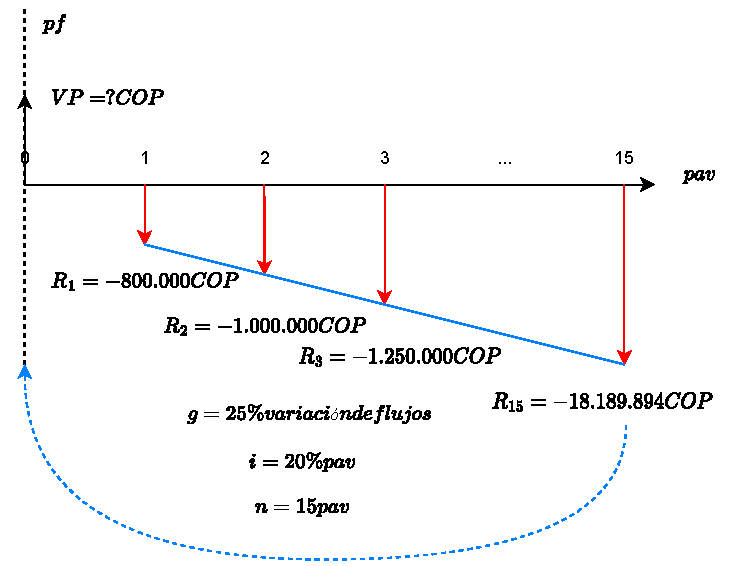
\includegraphics[trim=-5 -5 -5 -5 , scale=0.5]{6_Capitulo/img/ejemplos/8/Capitulo6Ejemplo8.pdf} }
		
		\\ \hline
		%%%%%%%%%%%%% FIN INSERCIÓN DE IMAGEN
		%%%%%FIN FLUJO DE CAJA
		
		%%%%% INICIO DECLARACIÓN FORMULAS
		%%%%%%%%%%% INICIO TITULO
		\rowcolor[HTML]{FFB183}
		\multicolumn{3}{|c|}{\cellcolor[HTML]{FFB183}\textbf{4. Declaración de fórmulas}}    \\ \hline
		%%%%%%%%%%% FIN TITULO
		%%%%%%%%%%% INICIO MATEMÁTICAS
		
		\multicolumn{3}{|c|}{$VP=(\frac{(R)[(1+g)^{n}(1+i)^{-n}-1]}{g-i}) \hspace{0.4 cm} \textit{Valor presente de un gradiente geometrico para } g \neq i$} \\ \hline
		
		%%%%%%%%%% FIN MATEMÁTICAS
		%%%%%% INICIO DESARROLLO MATEMÁTICO
		\rowcolor[HTML]{FFB183}
		%%%%%%%%%%INICIO TITULO
		\multicolumn{3}{|c|}{\cellcolor[HTML]{FFB183}\textbf{5. Desarrollo matemático}}       \\ \hline
		%%%%%%%%%% FIN TITULO
		%%%%%%%%%% INICIO MATEMÁTICAS
		
		\multicolumn{3}{|c|}{$VP=(\frac{( 800{.}000COP)[(1+0.25)^{15}(1+0,20)^{-15}-1]}{0.25-0.2}) \hspace{0.2 cm}\rightarrow \hspace{0.2 cm} VP=  13{.}515{.}591COP$} \\ \hline
		%%%%%%%%%% FIN MATEMÁTICAS
		%%%%%% FIN DESARROLLO MATEMÁTICO
		%%%%%% INICIO RESPUESTA
		\rowcolor[HTML]{FFB183}
		%%%%%%%%%%INICIO TITULO
		\multicolumn{3}{|c|}{\cellcolor[HTML]{FFB183}\textbf{6. Respuesta}}   \\ \hline
		%%%%%%%%%% FIN TITULO
		%%%%%%%%%% INICIO RESPUESTA MATEMÁTICA
		\multicolumn{3}{|c|}{${VP=  13{.}515{.}591COP}$} 
		\\ \hline
		%%%%%%%%%% FIN MATEMÁTICAS
		%%%%%% FIN RESPUESTA
	\end{longtable}
	%Se crean dos lineas en blanco para que no quede el siguiente texto tan pegado
	%\newline \newline %USARLO SI CREES QUE ES NECESARIO
\end{center}
%%%%%%%%%%%%%%%%%%%%%%%%%%FIN EJERCICIO 8 %%%%%%%%%%%%%%%%%%%%%%%%%%%
